\section{Estudi implementació \textit{mixer}}
S'ha considerat la possibilitat d'afegir un \textit{mixer} al turbofan calculat. El criteri de decisió és simple; si el \textit{mixer} millora l'empenta adimensinonal del rotor, i per tant redueix el consum específic, s'adoptarà. De no ser així, es mantindrà el motor sense mixer. Per fer els càlculs necessaris s'ha creat la funció \textit{mixer.m}. Aquesta té com a objectiu calcular les condicions del fluid a la sortida del mixer en funció de l'entrada a aquest dels dos fluxos, el primari i el secundari.
\begin{figure}[H]
	\centering
	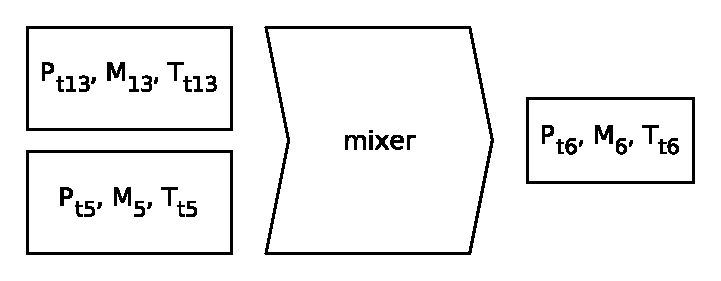
\includegraphics[scale=0.6]{./pics/mixer}
	\caption{Treball del mixer}
\end{figure}
Pel que fa a les propietats termodinàmiques que depenen de la temperatura, es fa una mitjana ponderada per tal de trobar-les a la sortida. A banda, com que s'està fent el disseny, s'imposa que el flux al mixer sigui laminar, de forma que les pèrdues siguin mínimes. Per fer això es prenen les següents hipòtesis:
\begin{itemize}
\item $M_5 = 1$
\item $P_5 = P_{13} = P_6$
\end{itemize}
Es tracta d'hipòtesis molt simplificatives que són poc realistes. Així doncs, es probable que donin problemes per trobar valors útils.

Per últim, es fa us de l'equació de quantitat de moviment:
\begin{equation}
\label{ccm}
F_6 = F_5 + F_{13}
\end{equation}
On:
\begin{equation}
F = \dot{m}\sqrt{\frac{RT_t}{\gamma\phi}}
\end{equation}
\begin{equation}
\label{phi}
\phi = \Bigg[ \frac{M\sqrt{1+\frac{\gamma-1}{2}M^2}}{a+\gamma M^2}\Bigg]^2
\end{equation}
Amb la Eq.\ref{ccm} es pot acabar traient el $M_6$ que servirà també per trobar $P_{t6}$. En el nostre cas, $M_6$ s'ha hagut de limitar a 1 doncs el mixer està ofegat.

A continuació es presenta la comparativa entre el motor sense mixer i amb mixer.
\begin{figure}[H]
	\centering
	\begin{tabular}{lc}
		\toprule[3pt]
		\textbf{Paràmetre}&\textbf{Valor}\\
		\midrule[1pt]
		$\hat{F}$ & 6.29 \\
		$\hat{F_{mixer}}$ & 3.14 \\
		\bottomrule[2pt]
	\end{tabular}
	\label{C_opti2}
	\caption{Comparativa mixer}
\end{figure}
Es pot concloure que el\textit{ mixer} perjudica al nostre motor doncs fa que sigui menys eficient. Així doncs,\textbf{ no s'emprarà mixer.}